\documentclass[tikz]{standalone}

\usepackage{tikz}
\usepackage{xcolor}
\usepackage{pgfplots}
\usepackage{siunitx}
\usepackage{fontspec}

\pgfplotsset{compat=1.18}

\usetikzlibrary{shapes,arrows,positioning,backgrounds,calc,intersections,calc,svg.path,fit}

\definecolor{ugent-re}{RGB}{220, 78, 40}        % vermilion			/ vermiljoen
\definecolor{ugent-we}{RGB}{45, 140, 168}       % no match

\begin{document}
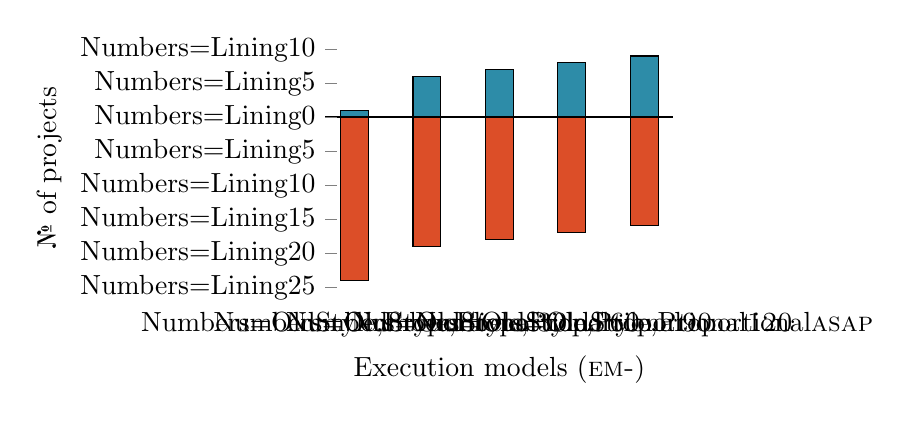
\begin{tikzpicture}
    \pgfplotsset{
        less/.style={fill=ugent-re},
        same/.style={fill=gray!30},
        more/.style={fill=ugent-we}
    }
    \begin{axis}[
        height=5cm,
        width=6cm,
        ybar stacked,
        symbolic x coords={30,60,90,120,asap},
        xtick distance=1,
        ytick distance=5,
        extra y ticks={0},
        extra y tick style={
            grid style={black,thick},
            yticklabel=\empty,
            ymajorgrids
        },
        axis on top,
        ylabel={№ of projects},
        xlabel={Execution models (\textsc{em-})},
        ytick pos=bottom,
        xtick style={draw=none},
        axis line style={draw=none},
        yticklabel={\pgfmathabs{\tick}\addfontfeature{Numbers={Lining}}\num[round-mode=places, round-precision=0]{\pgfmathresult}},
        xticklabel={\addfontfeature{Numbers={OldStyle,Proportional}}\textsc{\tick}}
    ]
        \addplot[less,forget plot] coordinates {
            (30,-24)
            (60,-19)
            (90,-18)
            (120,-17)
            (asap,-16)
        };
        \addplot[same,forget plot] coordinates {
            (30,0)
            (60,0)
            (90,0)
            (120,0)
            (asap,0)
        };
        \addplot[more,forget plot] coordinates {
            (30,1)
            (60,6)
            (90,7)
            (120,8)
            (asap,9)
        };
    \end{axis}
\end{tikzpicture}
\end{document}
